\documentclass[]{article}
\usepackage{lmodern}
\usepackage{amssymb,amsmath}
\usepackage{ifxetex,ifluatex}
\usepackage{fixltx2e} % provides \textsubscript
\ifnum 0\ifxetex 1\fi\ifluatex 1\fi=0 % if pdftex
  \usepackage[T1]{fontenc}
  \usepackage[utf8]{inputenc}
\else % if luatex or xelatex
  \ifxetex
    \usepackage{mathspec}
  \else
    \usepackage{fontspec}
  \fi
  \defaultfontfeatures{Ligatures=TeX,Scale=MatchLowercase}
\fi
% use upquote if available, for straight quotes in verbatim environments
\IfFileExists{upquote.sty}{\usepackage{upquote}}{}
% use microtype if available
\IfFileExists{microtype.sty}{%
\usepackage{microtype}
\UseMicrotypeSet[protrusion]{basicmath} % disable protrusion for tt fonts
}{}
\usepackage[margin=1in]{geometry}
\usepackage{hyperref}
\hypersetup{unicode=true,
            pdftitle={Stage 2: Exploratory Data Analysis},
            pdfauthor={Isaac Slagel and Jack Welsh},
            pdfborder={0 0 0},
            breaklinks=true}
\urlstyle{same}  % don't use monospace font for urls
\usepackage{color}
\usepackage{fancyvrb}
\newcommand{\VerbBar}{|}
\newcommand{\VERB}{\Verb[commandchars=\\\{\}]}
\DefineVerbatimEnvironment{Highlighting}{Verbatim}{commandchars=\\\{\}}
% Add ',fontsize=\small' for more characters per line
\usepackage{framed}
\definecolor{shadecolor}{RGB}{248,248,248}
\newenvironment{Shaded}{\begin{snugshade}}{\end{snugshade}}
\newcommand{\KeywordTok}[1]{\textcolor[rgb]{0.13,0.29,0.53}{\textbf{#1}}}
\newcommand{\DataTypeTok}[1]{\textcolor[rgb]{0.13,0.29,0.53}{#1}}
\newcommand{\DecValTok}[1]{\textcolor[rgb]{0.00,0.00,0.81}{#1}}
\newcommand{\BaseNTok}[1]{\textcolor[rgb]{0.00,0.00,0.81}{#1}}
\newcommand{\FloatTok}[1]{\textcolor[rgb]{0.00,0.00,0.81}{#1}}
\newcommand{\ConstantTok}[1]{\textcolor[rgb]{0.00,0.00,0.00}{#1}}
\newcommand{\CharTok}[1]{\textcolor[rgb]{0.31,0.60,0.02}{#1}}
\newcommand{\SpecialCharTok}[1]{\textcolor[rgb]{0.00,0.00,0.00}{#1}}
\newcommand{\StringTok}[1]{\textcolor[rgb]{0.31,0.60,0.02}{#1}}
\newcommand{\VerbatimStringTok}[1]{\textcolor[rgb]{0.31,0.60,0.02}{#1}}
\newcommand{\SpecialStringTok}[1]{\textcolor[rgb]{0.31,0.60,0.02}{#1}}
\newcommand{\ImportTok}[1]{#1}
\newcommand{\CommentTok}[1]{\textcolor[rgb]{0.56,0.35,0.01}{\textit{#1}}}
\newcommand{\DocumentationTok}[1]{\textcolor[rgb]{0.56,0.35,0.01}{\textbf{\textit{#1}}}}
\newcommand{\AnnotationTok}[1]{\textcolor[rgb]{0.56,0.35,0.01}{\textbf{\textit{#1}}}}
\newcommand{\CommentVarTok}[1]{\textcolor[rgb]{0.56,0.35,0.01}{\textbf{\textit{#1}}}}
\newcommand{\OtherTok}[1]{\textcolor[rgb]{0.56,0.35,0.01}{#1}}
\newcommand{\FunctionTok}[1]{\textcolor[rgb]{0.00,0.00,0.00}{#1}}
\newcommand{\VariableTok}[1]{\textcolor[rgb]{0.00,0.00,0.00}{#1}}
\newcommand{\ControlFlowTok}[1]{\textcolor[rgb]{0.13,0.29,0.53}{\textbf{#1}}}
\newcommand{\OperatorTok}[1]{\textcolor[rgb]{0.81,0.36,0.00}{\textbf{#1}}}
\newcommand{\BuiltInTok}[1]{#1}
\newcommand{\ExtensionTok}[1]{#1}
\newcommand{\PreprocessorTok}[1]{\textcolor[rgb]{0.56,0.35,0.01}{\textit{#1}}}
\newcommand{\AttributeTok}[1]{\textcolor[rgb]{0.77,0.63,0.00}{#1}}
\newcommand{\RegionMarkerTok}[1]{#1}
\newcommand{\InformationTok}[1]{\textcolor[rgb]{0.56,0.35,0.01}{\textbf{\textit{#1}}}}
\newcommand{\WarningTok}[1]{\textcolor[rgb]{0.56,0.35,0.01}{\textbf{\textit{#1}}}}
\newcommand{\AlertTok}[1]{\textcolor[rgb]{0.94,0.16,0.16}{#1}}
\newcommand{\ErrorTok}[1]{\textcolor[rgb]{0.64,0.00,0.00}{\textbf{#1}}}
\newcommand{\NormalTok}[1]{#1}
\usepackage{graphicx,grffile}
\makeatletter
\def\maxwidth{\ifdim\Gin@nat@width>\linewidth\linewidth\else\Gin@nat@width\fi}
\def\maxheight{\ifdim\Gin@nat@height>\textheight\textheight\else\Gin@nat@height\fi}
\makeatother
% Scale images if necessary, so that they will not overflow the page
% margins by default, and it is still possible to overwrite the defaults
% using explicit options in \includegraphics[width, height, ...]{}
\setkeys{Gin}{width=\maxwidth,height=\maxheight,keepaspectratio}
\IfFileExists{parskip.sty}{%
\usepackage{parskip}
}{% else
\setlength{\parindent}{0pt}
\setlength{\parskip}{6pt plus 2pt minus 1pt}
}
\setlength{\emergencystretch}{3em}  % prevent overfull lines
\providecommand{\tightlist}{%
  \setlength{\itemsep}{0pt}\setlength{\parskip}{0pt}}
\setcounter{secnumdepth}{0}
% Redefines (sub)paragraphs to behave more like sections
\ifx\paragraph\undefined\else
\let\oldparagraph\paragraph
\renewcommand{\paragraph}[1]{\oldparagraph{#1}\mbox{}}
\fi
\ifx\subparagraph\undefined\else
\let\oldsubparagraph\subparagraph
\renewcommand{\subparagraph}[1]{\oldsubparagraph{#1}\mbox{}}
\fi

%%% Use protect on footnotes to avoid problems with footnotes in titles
\let\rmarkdownfootnote\footnote%
\def\footnote{\protect\rmarkdownfootnote}

%%% Change title format to be more compact
\usepackage{titling}

% Create subtitle command for use in maketitle
\providecommand{\subtitle}[1]{
  \posttitle{
    \begin{center}\large#1\end{center}
    }
}

\setlength{\droptitle}{-2em}

  \title{Stage 2: Exploratory Data Analysis}
    \pretitle{\vspace{\droptitle}\centering\huge}
  \posttitle{\par}
    \author{Isaac Slagel and Jack Welsh}
    \preauthor{\centering\large\emph}
  \postauthor{\par}
      \predate{\centering\large\emph}
  \postdate{\par}
    \date{4/18/2019}

\usepackage{booktabs}
\usepackage{longtable}
\usepackage{array}
\usepackage{multirow}
\usepackage{wrapfig}
\usepackage{float}
\usepackage{colortbl}
\usepackage{pdflscape}
\usepackage{tabu}
\usepackage{threeparttable}
\usepackage{threeparttablex}
\usepackage[normalem]{ulem}
\usepackage{makecell}
\usepackage{xcolor}

\usepackage{dcolumn} \usepackage{float}

\begin{document}
\maketitle

\section{Main Report}\label{main-report}

\subsubsection{Pitbulls in Dallas
Shelters}\label{pitbulls-in-dallas-shelters}

In our EDA we found a distinct difference between outcomes for pitbulls
compared to other breeds of dogs. What we saw was that pitbulls tend to
be killed at a higher rate than other dogs. However we also found there
were other variables that influence the outcome of dogs like chip
status, outcome month, and intake condition. Inorder to quantify the
difference in treatment between dog breeds, we condensed our large
dataset into a smaller form and conducted a series of binomial
regressions described in Table 1.

\begin{table}[!htbp] \centering 
  \caption{Modeling Dog Outcomes in Dallas Animal Shelters} 
  \label{} 
\begin{tabular}{@{\extracolsep{5pt}}lD{.}{.}{-3} D{.}{.}{-3} D{.}{.}{-3} } 
\\[-1.8ex]\hline 
\hline \\[-1.8ex] 
 & \multicolumn{3}{c}{\textit{Dependent variable:}} \\ 
\cline{2-4} 
\\[-1.8ex] & \multicolumn{3}{c}{Proportion of dogs who died} \\ 
\\[-1.8ex] & \multicolumn{1}{c}{(1)} & \multicolumn{1}{c}{(2)} & \multicolumn{1}{c}{(3)}\\ 
\hline \\[-1.8ex] 
 Intercept & 0.116^{***} & 0.111^{***} & 0.552^{***} \\ 
  & \multicolumn{1}{c}{(0.069$, $0.186)} & \multicolumn{1}{c}{(0.069$, $0.170)} & \multicolumn{1}{c}{(0.454$, $0.669)} \\ 
  & & & \\ 
 Pitbull & 3.440^{***} & 3.424^{***} & 3.489^{***} \\ 
  & \multicolumn{1}{c}{(1.795$, $6.557)} & \multicolumn{1}{c}{(1.905$, $6.130)} & \multicolumn{1}{c}{(3.022$, $4.027)} \\ 
  & & & \\ 
 Scannable Chip & 0.789 & 0.799 & 0.781^{***} \\ 
  & \multicolumn{1}{c}{(0.377$, $1.566)} & \multicolumn{1}{c}{(0.412$, $1.483)} & \multicolumn{1}{c}{(0.667$, $0.911)} \\ 
  & & & \\ 
 Summer Outcome & 1.461 & 1.447 & 1.478^{***} \\ 
  & \multicolumn{1}{c}{(0.725$, $2.852)} & \multicolumn{1}{c}{(0.771$, $2.649)} & \multicolumn{1}{c}{(1.271$, $1.718)} \\ 
  & & & \\ 
 Contagious &  & 7.286^{**} & 3.975^{***} \\ 
  &  & \multicolumn{1}{c}{(1.324$, $44.137)} & \multicolumn{1}{c}{(2.568$, $6.168)} \\ 
  & & & \\ 
 Treatable At Intake &  &  & 0.161^{***} \\ 
  &  &  & \multicolumn{1}{c}{(0.133$, $0.196)} \\ 
  & & & \\ 
\hline \\[-1.8ex] 
Overdisperson Parameter & 139.72 & 111.46 & 6.27 \\ 
Nested F Test &  & F: 5.1142^* & F: 313.62^{***} \\ 
\hline 
\hline \\[-1.8ex] 
\textit{Note:}  & \multicolumn{3}{r}{$^{*}$p$<$0.1; $^{**}$p$<$0.05; $^{***}$p$<$0.01} \\ 
\end{tabular} 
\end{table}

We see in Table 1 that all of our models have variable estimates that
are significant including Model 3 which accounted for whether or not an
animal was deemed ``treatable'' at the time of intake. Further, by two F
tests we see each of our models is an improvement on the one before it
(Model 1 \(\rightarrow\) Model 2: F = 5.1141, p-value = 0.031) (Model 2
\(\rightarrow\) Model 3: F = 313.62, p-value
\textless{}\textless{}\textless{} .05). Before our final draft we will
continue to explore these trends and look for other variables that
contribute to dog outcomes.

Using model 3 as our best model of dog outcomes from the animal shelter,
we glean several insights about how certain characteristics of dogs have
relationships with those animal's outcome from the animal shelter. For
instance, if a dog is a pitbull, we expect it's odds of leaving the
animal shelter dead increase by 348\%, after controlling for chip
status, season, and intake condition. Yikes! On the other hand, if a dog
comes into the shelter with a scannable chip, we expect the animals odds
of dying within the shelter system to drop by about 22\%, after
controlling for pitbull, season, and intake condition. Interestingly
enough, if a dog has its outcome in the summer, the odds of that outcome
being death are about 47\% higher, controlling for breed, chip status,
and intake condition.

One interesting issue that we encountered in this section of our
modeling was the significance of the dataset we fit on SE estimates. If
we summarized our data for each specific model, parameter estimates had
increased SEs and more insignificant p-values. However, if we fit all of
our models on the same, more extensive, summary table, SEs were small
and parameters were more likely to be significant. We decided to proceed
with the latter option, as it allows us to carry out nested F tests and
would be more like a modeling process for true grouped data. This could
mean that our SEs are artifically low.

\subsubsection{Dogs and Cats}\label{dogs-and-cats}

Interestingly enough, we were not able to find any significant
relationships between dog and cat outcomes. We tried multiple binomial
models accounting for stray, summer, and chip status. None of these
models showed any significance. This suprised us a lot, as we saw a few
trends in our EDA and have heard stories about poorer outcomes for cats
in animal shelters. We may consider looking into a few other outcomes
for our final report (we only considered death at outcome).

\subsubsection{Conrtrolling for City Council
District}\label{conrtrolling-for-city-council-district}

To control for differnces between city council districts we chose to use
multilevel logistic regresison. We began by fitting two random
intercepts models with no level 1 or level 2 terms, one for adopted as
the response and one for death within the shelter system as a response.

While looking at adoptions as our response we found that our one fixed
effect \(\alpha_0=-0.4930\), which if you exponentiate and convert to a
proportion we see that the average proportion of dogs being adopted is
0.379. It is sad to think that only about one out of every three dogs
gets adopted. We fonud a \(\sigma_u=0.2438\) so the average deviance
between city council districts 0.2438.

Next we repeated the same model with out\_dead as the outcome. We fonud
a fixed effect for our \(\alpha_0=-1.65465\), which after you
exponentiate and convert to a proportion we get 0.160. So only 16\% of
the dogs that enter the animal shelter system exit dead. We found a
\(\sigma_u=0.1395\), so the average deciance between city council
districts is 0.1395.

\begin{Shaded}
\begin{Highlighting}[]
\KeywordTok{stargazer}\NormalTok{(mod.1_dead, mod.}\DecValTok{1}\NormalTok{,}
          \DataTypeTok{add.lines =} \KeywordTok{list}\NormalTok{(}\KeywordTok{c}\NormalTok{(}\StringTok{"Between District $}\CharTok{\textbackslash{}\textbackslash{}}\StringTok{sigma$"}\NormalTok{, }\StringTok{"0.1395"}\NormalTok{, }\StringTok{"0.1408"}\NormalTok{)),}
          \DataTypeTok{title=}\StringTok{"Predicting Dead Outcomes and Adopted outcomes with Multilevel Structure No level 1 Predictors"}\NormalTok{,}
          \DataTypeTok{type=}\StringTok{'latex'}\NormalTok{,}
          \DataTypeTok{align=}\OtherTok{TRUE}\NormalTok{,}
          \DataTypeTok{header=}\OtherTok{FALSE}\NormalTok{,}
          \DataTypeTok{intercept.bottom =} \OtherTok{FALSE}\NormalTok{)}
\end{Highlighting}
\end{Shaded}

\begin{table}[!htbp] \centering 
  \caption{Predicting Dead Outcomes and Adopted outcomes with Multilevel Structure No level 1 Predictors} 
  \label{} 
\begin{tabular}{@{\extracolsep{5pt}}lD{.}{.}{-3} D{.}{.}{-3} } 
\\[-1.8ex]\hline 
\hline \\[-1.8ex] 
 & \multicolumn{2}{c}{\textit{Dependent variable:}} \\ 
\cline{2-3} 
\\[-1.8ex] & \multicolumn{1}{c}{out\_dead} & \multicolumn{1}{c}{adopted} \\ 
\\[-1.8ex] & \multicolumn{1}{c}{(1)} & \multicolumn{1}{c}{(2)}\\ 
\hline \\[-1.8ex] 
 Constant & -1.655^{***} & -0.493^{***} \\ 
  & (0.041) & (0.067) \\ 
  & & \\ 
\hline \\[-1.8ex] 
Between District $\sigma$ & 0.1395 & 0.1408 \\ 
Observations & \multicolumn{1}{c}{45,487} & \multicolumn{1}{c}{45,487} \\ 
Log Likelihood & \multicolumn{1}{c}{-19,759.010} & \multicolumn{1}{c}{-29,340.940} \\ 
Akaike Inf. Crit. & \multicolumn{1}{c}{39,522.010} & \multicolumn{1}{c}{58,685.880} \\ 
Bayesian Inf. Crit. & \multicolumn{1}{c}{39,539.460} & \multicolumn{1}{c}{58,703.330} \\ 
\hline 
\hline \\[-1.8ex] 
\textit{Note:}  & \multicolumn{2}{r}{$^{*}$p$<$0.1; $^{**}$p$<$0.05; $^{***}$p$<$0.01} \\ 
\end{tabular} 
\end{table}

We repeated the same procedure as above just this time adding in summer,
chip status and treatable intake. We found with adopted as the response
the average proportion adopted is 0.126 not durring the summer for dogs
that are untreatable and the chip was not readable or not present. We
found that all of our predictors are significant, see table. We fonud
that the summer on average increase the odds of a dog being adopted by
7.4\% compared not during the summer controlling for chip status, and
treatable intake. Suprisingly we fonud that if a dog has a readable chip
on average the odds of them being adopted decreases by 11.5\% compared
to a dog with a unreadable chip or no chip controlling for summer and
treatable intake. This suprised us at first, but then we realized that
dogs that have a chip tend to be dogs that are returned to owner.
Unsuprisingly, a dog with a treatable intake odds of being adopted are
393\% higher than dogs without a treatable intake controlling for
whether it is summer and chip status.

When looking at death as our response we found that the average
proportion of dogs dying in the animal shelter system not durring the
summer, without a chip, and with a non treateable intake is 0.52. We
found that on average summer increases the odds of death increase by
45.5\% controlling for chip status and treatable intake. On average
having a chip decreases the odds of death by 21\% acconuting for summer
and treatable intake. On average treatable intake decreases the odds of
death ny 89.3\% accounting for summer and chip status.

\begin{Shaded}
\begin{Highlighting}[]
\KeywordTok{stargazer}\NormalTok{(mod.}\FloatTok{2.}\NormalTok{dead, mod.}\FloatTok{2.}\NormalTok{adopted,}
          \DataTypeTok{add.lines =} \KeywordTok{list}\NormalTok{(}\KeywordTok{c}\NormalTok{(}\StringTok{"Between District $}\CharTok{\textbackslash{}\textbackslash{}}\StringTok{sigma$"}\NormalTok{, }\StringTok{"0.2438"}\NormalTok{, }\StringTok{"0.2896"}\NormalTok{)),}
          \DataTypeTok{title=}\StringTok{"Predicting Dead Outcomes and Adoption Outcomes with Multilevel Structure with Level 2 Predictors"}\NormalTok{,}
          \DataTypeTok{type=}\StringTok{'latex'}\NormalTok{,}
          \DataTypeTok{align=}\OtherTok{TRUE}\NormalTok{,}
          \DataTypeTok{header=}\OtherTok{FALSE}\NormalTok{,}
          \DataTypeTok{intercept.bottom =} \OtherTok{FALSE}\NormalTok{)}
\end{Highlighting}
\end{Shaded}

\begin{table}[!htbp] \centering 
  \caption{Predicting Dead Outcomes and Adoption Outcomes with Multilevel Structure with Level 2 Predictors} 
  \label{} 
\begin{tabular}{@{\extracolsep{5pt}}lD{.}{.}{-3} D{.}{.}{-3} } 
\\[-1.8ex]\hline 
\hline \\[-1.8ex] 
 & \multicolumn{2}{c}{\textit{Dependent variable:}} \\ 
\cline{2-3} 
\\[-1.8ex] & \multicolumn{1}{c}{out\_dead} & \multicolumn{1}{c}{adopted} \\ 
\\[-1.8ex] & \multicolumn{1}{c}{(1)} & \multicolumn{1}{c}{(2)}\\ 
\hline \\[-1.8ex] 
 Constant & 0.083 & -1.936^{***} \\ 
  & (0.053) & (0.093) \\ 
  & & \\ 
 summer & 0.375^{***} & 0.072^{***} \\ 
  & (0.030) & (0.023) \\ 
  & & \\ 
 chip\_status & -0.236^{***} & -0.122^{***} \\ 
  & (0.031) & (0.022) \\ 
  & & \\ 
 treatable\_intake & -2.121^{***} & 1.597^{***} \\ 
  & (0.036) & (0.051) \\ 
  & & \\ 
\hline \\[-1.8ex] 
Between District $\sigma$ & 0.2438 & 0.2896 \\ 
Observations & \multicolumn{1}{c}{45,487} & \multicolumn{1}{c}{45,487} \\ 
Log Likelihood & \multicolumn{1}{c}{-17,995.950} & \multicolumn{1}{c}{-28,653.040} \\ 
Akaike Inf. Crit. & \multicolumn{1}{c}{36,001.900} & \multicolumn{1}{c}{57,316.070} \\ 
Bayesian Inf. Crit. & \multicolumn{1}{c}{36,045.530} & \multicolumn{1}{c}{57,359.700} \\ 
\hline 
\hline \\[-1.8ex] 
\textit{Note:}  & \multicolumn{2}{r}{$^{*}$p$<$0.1; $^{**}$p$<$0.05; $^{***}$p$<$0.01} \\ 
\end{tabular} 
\end{table}

\section{Annotated Appendix}\label{annotated-appendix}

\subsubsection{Pitbulls}\label{pitbulls}

One of our research interests was to look into how different species of
dogs fare in the animal shelter system. Specifically, we were interested
in why pitbulls are more likely to be dead at the outcome of their time
in the shelter. Does this trend continue after controlling for other
variables in our dataset?

Initially we fit a model which factors in the chip status, whether or
not the outcome was in the summer, and whether the dog was a pitbull or
not.

\begin{Shaded}
\begin{Highlighting}[]
\NormalTok{pitbull_binom <-}\StringTok{ }\NormalTok{adoptions }\OperatorTok
\StringTok{  }\KeywordTok{filter}\NormalTok{(}\OperatorTok{!}\KeywordTok{str_detect}\NormalTok{(intake_subtype, }\StringTok{"(DEAD)|(DIED)"}\NormalTok{)) }\OperatorTok
\StringTok{  }\KeywordTok{filter}\NormalTok{(dog }\OperatorTok{==}\StringTok{ }\DecValTok{1}\NormalTok{) }\OperatorTok
\StringTok{  }\KeywordTok{mutate}\NormalTok{(}\DataTypeTok{out_dead =}\NormalTok{ outcome_type }\OperatorTok\StringTok{ }\KeywordTok{c}\NormalTok{(}\StringTok{"DEAD ON ARRIVAL"}\NormalTok{, }\StringTok{"EUTHANIZED"}\NormalTok{, }\StringTok{"DIED"}\NormalTok{),}
         \DataTypeTok{summer =} \KeywordTok{ifelse}\NormalTok{(month }\OperatorTok\StringTok{ }\KeywordTok{c}\NormalTok{(}\DecValTok{5}\NormalTok{, }\DecValTok{6}\NormalTok{, }\DecValTok{7}\NormalTok{, }\DecValTok{8}\NormalTok{, }\DecValTok{9}\NormalTok{), }\DecValTok{1}\NormalTok{, }\DecValTok{0}\NormalTok{)) }\OperatorTok
\StringTok{  }\KeywordTok{mutate}\NormalTok{(}\DataTypeTok{chip_status =} \KeywordTok{ifelse}\NormalTok{(chip_status}\OperatorTok{==}\StringTok{"SCAN CHIP"}\NormalTok{, }\DecValTok{1}\NormalTok{, }\DecValTok{0}\NormalTok{)) }\OperatorTok
\StringTok{  }\KeywordTok{group_by}\NormalTok{(pitbull, chip_status, summer, month) }\OperatorTok
\StringTok{  }\KeywordTok{summarize}\NormalTok{(}\DataTypeTok{prop_dead =} \KeywordTok{sum}\NormalTok{(out_dead)}\OperatorTok{/}\KeywordTok{n}\NormalTok{(), }\DataTypeTok{count =} \KeywordTok{n}\NormalTok{())}


\NormalTok{pitbull_model1_binom <-}\StringTok{ }\KeywordTok{glm}\NormalTok{(prop_dead }\OperatorTok{~}\StringTok{ }\NormalTok{pitbull }\OperatorTok{+}\StringTok{ }\NormalTok{chip_status }\OperatorTok{+}\StringTok{ }\NormalTok{summer , }\DataTypeTok{weights =}\NormalTok{ count, }\DataTypeTok{family =}\NormalTok{ binomial, }\DataTypeTok{data =}\NormalTok{ pitbull_binom)}

\NormalTok{pitbull_model1_quasi <-}\StringTok{ }\KeywordTok{glm}\NormalTok{(prop_dead }\OperatorTok{~}\StringTok{ }\NormalTok{pitbull }\OperatorTok{+}\StringTok{ }\NormalTok{chip_status }\OperatorTok{+}\StringTok{ }\NormalTok{summer , }\DataTypeTok{weights =}\NormalTok{ count, }\DataTypeTok{family =}\NormalTok{ quasibinomial, }\DataTypeTok{data =}\NormalTok{ pitbull_binom)}

\KeywordTok{summary}\NormalTok{(pitbull_model1_binom)}
\end{Highlighting}
\end{Shaded}

\begin{verbatim}
## 
## Call:
## glm(formula = prop_dead ~ pitbull + chip_status + summer, family = binomial, 
##     data = pitbull_binom, weights = count)
## 
## Deviance Residuals: 
##     Min       1Q   Median       3Q      Max  
## -7.4184  -1.8174  -0.4575   1.5859   9.4807  
## 
## Coefficients:
##             Estimate Std. Error  z value Pr(>|z|)    
## (Intercept) -2.15259    0.02131 -100.994  < 2e-16 ***
## pitbull      1.23537    0.02783   44.387  < 2e-16 ***
## chip_status -0.23649    0.03050   -7.753 8.97e-15 ***
## summer       0.37879    0.02938   12.891  < 2e-16 ***
## ---
## Signif. codes:  0 '***' 0.001 '**' 0.01 '*' 0.05 '.' 0.1 ' ' 1
## 
## (Dispersion parameter for binomial family taken to be 1)
## 
##     Null deviance: 2641.29  on 51  degrees of freedom
## Residual deviance:  544.19  on 48  degrees of freedom
##   (2 observations deleted due to missingness)
## AIC: 867.48
## 
## Number of Fisher Scoring iterations: 4
\end{verbatim}

\begin{Shaded}
\begin{Highlighting}[]
\KeywordTok{exp}\NormalTok{(}\KeywordTok{confint}\NormalTok{(pitbull_model1_binom))}
\end{Highlighting}
\end{Shaded}

\begin{verbatim}
## Waiting for profiling to be done...
\end{verbatim}

\begin{verbatim}
##                 2.5 %    97.5 %
## (Intercept) 0.1114096 0.1211179
## pitbull     3.2569778 3.6324244
## chip_status 0.7434426 0.8378715
## summer      1.3786281 1.5469365
\end{verbatim}

\begin{Shaded}
\begin{Highlighting}[]
\KeywordTok{summary}\NormalTok{(pitbull_model1_quasi)}
\end{Highlighting}
\end{Shaded}

\begin{verbatim}
## 
## Call:
## glm(formula = prop_dead ~ pitbull + chip_status + summer, family = quasibinomial, 
##     data = pitbull_binom, weights = count)
## 
## Deviance Residuals: 
##     Min       1Q   Median       3Q      Max  
## -7.4184  -1.8174  -0.4575   1.5859   9.4807  
## 
## Coefficients:
##             Estimate Std. Error t value Pr(>|t|)    
## (Intercept) -2.15259    0.06971 -30.880  < 2e-16 ***
## pitbull      1.23537    0.09103  13.572  < 2e-16 ***
## chip_status -0.23649    0.09976  -2.371 0.021826 *  
## summer       0.37879    0.09610   3.942 0.000262 ***
## ---
## Signif. codes:  0 '***' 0.001 '**' 0.01 '*' 0.05 '.' 0.1 ' ' 1
## 
## (Dispersion parameter for quasibinomial family taken to be 10.69677)
## 
##     Null deviance: 2641.29  on 51  degrees of freedom
## Residual deviance:  544.19  on 48  degrees of freedom
##   (2 observations deleted due to missingness)
## AIC: NA
## 
## Number of Fisher Scoring iterations: 4
\end{verbatim}

\begin{Shaded}
\begin{Highlighting}[]
\KeywordTok{exp}\NormalTok{(}\KeywordTok{confint}\NormalTok{(pitbull_model1_quasi))}
\end{Highlighting}
\end{Shaded}

\begin{verbatim}
## Waiting for profiling to be done...
\end{verbatim}

\begin{verbatim}
##                 2.5 %    97.5 %
## (Intercept) 0.1011467 0.1329404
## pitbull     2.8769183 4.1109439
## chip_status 0.6478111 0.9580232
## summer      1.2082342 1.7612914
\end{verbatim}

Initially we see that all variables included have a significant
relationship to the proportion of dogs who are dead at the end of their
time in the shelter, even after inflating our standard errors to account
for the variance structure of our data.

Next lets try to control for whether or not a animal was contagious when
it was brought into the shelter.

\begin{Shaded}
\begin{Highlighting}[]
\NormalTok{pitbull_binom <-}\StringTok{ }\NormalTok{adoptions }\OperatorTok
\StringTok{  }\KeywordTok{filter}\NormalTok{(}\OperatorTok{!}\KeywordTok{str_detect}\NormalTok{(intake_subtype, }\StringTok{"(DEAD)|(DIED)"}\NormalTok{)) }\OperatorTok
\StringTok{  }\KeywordTok{filter}\NormalTok{(dog }\OperatorTok{==}\StringTok{ }\DecValTok{1}\NormalTok{) }\OperatorTok
\StringTok{  }\KeywordTok{mutate}\NormalTok{(}\DataTypeTok{out_dead =}\NormalTok{ outcome_type }\OperatorTok\StringTok{ }\KeywordTok{c}\NormalTok{(}\StringTok{"DEAD ON ARRIVAL"}\NormalTok{, }\StringTok{"EUTHANIZED"}\NormalTok{, }\StringTok{"DIED"}\NormalTok{),}
         \DataTypeTok{summer =} \KeywordTok{ifelse}\NormalTok{(month }\OperatorTok\StringTok{ }\KeywordTok{c}\NormalTok{(}\DecValTok{5}\NormalTok{, }\DecValTok{6}\NormalTok{, }\DecValTok{7}\NormalTok{, }\DecValTok{8}\NormalTok{, }\DecValTok{9}\NormalTok{), }\DecValTok{1}\NormalTok{, }\DecValTok{0}\NormalTok{),}
         \DataTypeTok{chip_status =} \KeywordTok{ifelse}\NormalTok{(chip_status}\OperatorTok{==}\StringTok{"SCAN CHIP"}\NormalTok{, }\DecValTok{1}\NormalTok{, }\DecValTok{0}\NormalTok{),}
         \DataTypeTok{contagious=}\KeywordTok{ifelse}\NormalTok{(}\KeywordTok{grepl}\NormalTok{(}\StringTok{".*[^NON-]CONTAGIOUS"}\NormalTok{, intake_condition),}\DecValTok{1}\NormalTok{,}\DecValTok{0}\NormalTok{)) }\OperatorTok
\StringTok{  }\KeywordTok{group_by}\NormalTok{(pitbull, chip_status, summer, contagious) }\OperatorTok
\StringTok{  }\KeywordTok{summarize}\NormalTok{(}\DataTypeTok{prop_dead =} \KeywordTok{sum}\NormalTok{(out_dead)}\OperatorTok{/}\KeywordTok{n}\NormalTok{(), }\DataTypeTok{count =} \KeywordTok{n}\NormalTok{())}

\NormalTok{pitbull_model2_binom <-}\StringTok{ }\KeywordTok{glm}\NormalTok{(prop_dead }\OperatorTok{~}\StringTok{ }\NormalTok{pitbull }\OperatorTok{+}\StringTok{ }\NormalTok{chip_status }\OperatorTok{+}
\StringTok{                      }\NormalTok{summer }\OperatorTok{+}\StringTok{ }\NormalTok{contagious, }\DataTypeTok{weights =}\NormalTok{ count,}
                    \DataTypeTok{family =}\NormalTok{ binomial, }\DataTypeTok{data =}\NormalTok{ pitbull_binom)}

\NormalTok{pitbull_model2_quasi <-}\StringTok{ }\KeywordTok{glm}\NormalTok{(prop_dead }\OperatorTok{~}\StringTok{ }\NormalTok{pitbull }\OperatorTok{+}\StringTok{ }\NormalTok{chip_status }\OperatorTok{+}
\StringTok{                      }\NormalTok{summer }\OperatorTok{+}\StringTok{ }\NormalTok{contagious , }\DataTypeTok{weights =}\NormalTok{ count,}
                    \DataTypeTok{family =}\NormalTok{ quasibinomial, }\DataTypeTok{data =}\NormalTok{ pitbull_binom)}

\KeywordTok{summary}\NormalTok{(pitbull_model2_binom)}
\end{Highlighting}
\end{Shaded}

\begin{verbatim}
## 
## Call:
## glm(formula = prop_dead ~ pitbull + chip_status + summer + contagious, 
##     family = binomial, data = pitbull_binom, weights = count)
## 
## Deviance Residuals: 
##      Min        1Q    Median        3Q       Max  
## -2.89655  -1.32251  -0.08517   1.08867   2.12765  
## 
## Coefficients:
##             Estimate Std. Error  z value Pr(>|z|)    
## (Intercept) -2.20165    0.02169 -101.518  < 2e-16 ***
## pitbull      1.23078    0.02814   43.742  < 2e-16 ***
## chip_status -0.22483    0.03077   -7.306 2.74e-13 ***
## summer       0.36978    0.02969   12.456  < 2e-16 ***
## contagious   1.98593    0.08113   24.477  < 2e-16 ***
## ---
## Signif. codes:  0 '***' 0.001 '**' 0.01 '*' 0.05 '.' 0.1 ' ' 1
## 
## (Dispersion parameter for binomial family taken to be 1)
## 
##     Null deviance: 2699.882  on 15  degrees of freedom
## Residual deviance:   32.758  on 11  degrees of freedom
##   (2 observations deleted due to missingness)
## AIC: 143.79
## 
## Number of Fisher Scoring iterations: 3
\end{verbatim}

\begin{Shaded}
\begin{Highlighting}[]
\KeywordTok{exp}\NormalTok{(}\KeywordTok{confint}\NormalTok{(pitbull_model2_binom))}
\end{Highlighting}
\end{Shaded}

\begin{verbatim}
## Waiting for profiling to be done...
\end{verbatim}

\begin{verbatim}
##                 2.5 %    97.5 %
## (Intercept) 0.1059964 0.1154017
## pitbull     3.2401347 3.6179798
## chip_status 0.7517627 0.8481433
## summer      1.3654369 1.5339545
## contagious  6.2166833 8.5454709
\end{verbatim}

\begin{Shaded}
\begin{Highlighting}[]
\KeywordTok{summary}\NormalTok{(pitbull_model2_quasi)}
\end{Highlighting}
\end{Shaded}

\begin{verbatim}
## 
## Call:
## glm(formula = prop_dead ~ pitbull + chip_status + summer + contagious, 
##     family = quasibinomial, data = pitbull_binom, weights = count)
## 
## Deviance Residuals: 
##      Min        1Q    Median        3Q       Max  
## -2.89655  -1.32251  -0.08517   1.08867   2.12765  
## 
## Coefficients:
##             Estimate Std. Error t value Pr(>|t|)    
## (Intercept) -2.20165    0.03766 -58.455 4.54e-15 ***
## pitbull      1.23078    0.04887  25.187 4.45e-11 ***
## chip_status -0.22483    0.05344  -4.207  0.00147 ** 
## summer       0.36978    0.05156   7.172 1.82e-05 ***
## contagious   1.98593    0.14091  14.094 2.19e-08 ***
## ---
## Signif. codes:  0 '***' 0.001 '**' 0.01 '*' 0.05 '.' 0.1 ' ' 1
## 
## (Dispersion parameter for quasibinomial family taken to be 3.01608)
## 
##     Null deviance: 2699.882  on 15  degrees of freedom
## Residual deviance:   32.758  on 11  degrees of freedom
##   (2 observations deleted due to missingness)
## AIC: NA
## 
## Number of Fisher Scoring iterations: 3
\end{verbatim}

\begin{Shaded}
\begin{Highlighting}[]
\KeywordTok{exp}\NormalTok{(}\KeywordTok{confint}\NormalTok{(pitbull_model2_quasi))}
\end{Highlighting}
\end{Shaded}

\begin{verbatim}
## Waiting for profiling to be done...
\end{verbatim}

\begin{verbatim}
##                 2.5 %    97.5 %
## (Intercept) 0.1026891 0.1190278
## pitbull     3.1110085 3.7678996
## chip_status 0.7188083 0.8863497
## summer      1.3078316 1.6007855
## contagious  5.5323688 9.6176550
\end{verbatim}

Next lets try to control for whether or not a animal was treatable when
it was brought into the shelter.

\begin{Shaded}
\begin{Highlighting}[]
\NormalTok{pitbull_binom <-}\StringTok{ }\NormalTok{adoptions }\OperatorTok
\StringTok{  }\KeywordTok{filter}\NormalTok{(}\OperatorTok{!}\KeywordTok{str_detect}\NormalTok{(intake_subtype, }\StringTok{"(DEAD)|(DIED)"}\NormalTok{)) }\OperatorTok
\StringTok{  }\KeywordTok{filter}\NormalTok{(dog }\OperatorTok{==}\StringTok{ }\DecValTok{1}\NormalTok{) }\OperatorTok
\StringTok{  }\KeywordTok{mutate}\NormalTok{(}\DataTypeTok{out_dead =}\NormalTok{ outcome_type }\OperatorTok\StringTok{ }\KeywordTok{c}\NormalTok{(}\StringTok{"DEAD ON ARRIVAL"}\NormalTok{, }\StringTok{"EUTHANIZED"}\NormalTok{, }\StringTok{"DIED"}\NormalTok{),}
         \DataTypeTok{summer =} \KeywordTok{ifelse}\NormalTok{(month }\OperatorTok\StringTok{ }\KeywordTok{c}\NormalTok{(}\DecValTok{5}\NormalTok{, }\DecValTok{6}\NormalTok{, }\DecValTok{7}\NormalTok{, }\DecValTok{8}\NormalTok{, }\DecValTok{9}\NormalTok{), }\DecValTok{1}\NormalTok{, }\DecValTok{0}\NormalTok{),}
         \DataTypeTok{chip_status =} \KeywordTok{ifelse}\NormalTok{(chip_status}\OperatorTok{==}\StringTok{"SCAN CHIP"}\NormalTok{, }\DecValTok{1}\NormalTok{, }\DecValTok{0}\NormalTok{),}
         \DataTypeTok{contagious=}\KeywordTok{ifelse}\NormalTok{(}\KeywordTok{grepl}\NormalTok{(}\StringTok{".*[^NON-]CONTAGIOUS"}\NormalTok{, intake_condition),}\DecValTok{1}\NormalTok{,}\DecValTok{0}\NormalTok{),}
         \DataTypeTok{treatable=}\KeywordTok{ifelse}\NormalTok{(}\KeywordTok{grepl}\NormalTok{(}\StringTok{"^TREATABLE.*"}\NormalTok{, intake_condition),}\DecValTok{1}\NormalTok{,}\DecValTok{0}\NormalTok{)) }\OperatorTok
\StringTok{  }\KeywordTok{group_by}\NormalTok{(pitbull, chip_status, summer, month, contagious, treatable) }\OperatorTok
\StringTok{  }\KeywordTok{summarize}\NormalTok{(}\DataTypeTok{prop_dead =} \KeywordTok{sum}\NormalTok{(out_dead)}\OperatorTok{/}\KeywordTok{n}\NormalTok{(), }\DataTypeTok{count =} \KeywordTok{n}\NormalTok{())}

\NormalTok{pitbull_model3_binom <-}\StringTok{ }\KeywordTok{glm}\NormalTok{(prop_dead }\OperatorTok{~}\StringTok{ }\NormalTok{pitbull }\OperatorTok{+}\StringTok{ }\NormalTok{chip_status }\OperatorTok{+}
\StringTok{                      }\NormalTok{summer }\OperatorTok{+}\StringTok{ }\NormalTok{contagious }\OperatorTok{+}\StringTok{ }\NormalTok{treatable, }\DataTypeTok{weights =}\NormalTok{ count,}
                    \DataTypeTok{family =}\NormalTok{ binomial, }\DataTypeTok{data =}\NormalTok{ pitbull_binom)}

\NormalTok{pitbull_model3_quasi <-}\StringTok{ }\KeywordTok{glm}\NormalTok{(prop_dead }\OperatorTok{~}\StringTok{ }\NormalTok{pitbull }\OperatorTok{+}\StringTok{ }\NormalTok{chip_status }\OperatorTok{+}
\StringTok{                      }\NormalTok{summer }\OperatorTok{+}\StringTok{ }\NormalTok{contagious }\OperatorTok{+}\StringTok{ }\NormalTok{treatable,}
                      \DataTypeTok{weights =}\NormalTok{ count,}
                      \DataTypeTok{family =}\NormalTok{ quasibinomial, }\DataTypeTok{data =}\NormalTok{ pitbull_binom)}

\KeywordTok{summary}\NormalTok{(pitbull_model3_binom)}
\end{Highlighting}
\end{Shaded}

\begin{verbatim}
## 
## Call:
## glm(formula = prop_dead ~ pitbull + chip_status + summer + contagious + 
##     treatable, family = binomial, data = pitbull_binom, weights = count)
## 
## Deviance Residuals: 
##     Min       1Q   Median       3Q      Max  
## -6.0491  -1.4236  -0.1897   0.9336   9.5936  
## 
## Coefficients:
##             Estimate Std. Error z value Pr(>|z|)    
## (Intercept) -0.59457    0.03949  -15.06  < 2e-16 ***
## pitbull      1.24955    0.02925   42.72  < 2e-16 ***
## chip_status -0.24774    0.03176   -7.80 6.21e-15 ***
## summer       0.39095    0.03070   12.73  < 2e-16 ***
## contagious   1.38010    0.08913   15.48  < 2e-16 ***
## treatable   -1.82378    0.03953  -46.14  < 2e-16 ***
## ---
## Signif. codes:  0 '***' 0.001 '**' 0.01 '*' 0.05 '.' 0.1 ' ' 1
## 
## (Dispersion parameter for binomial family taken to be 1)
## 
##     Null deviance: 5475.42  on 194  degrees of freedom
## Residual deviance:  842.76  on 189  degrees of freedom
##   (2 observations deleted due to missingness)
## AIC: 1514.1
## 
## Number of Fisher Scoring iterations: 4
\end{verbatim}

\begin{Shaded}
\begin{Highlighting}[]
\KeywordTok{exp}\NormalTok{(}\KeywordTok{confint}\NormalTok{(pitbull_model3_binom))}
\end{Highlighting}
\end{Shaded}

\begin{verbatim}
## Waiting for profiling to be done...
\end{verbatim}

\begin{verbatim}
##                 2.5 %    97.5 %
## (Intercept) 0.5106406 0.5961339
## pitbull     3.2943807 3.6946299
## chip_status 0.7333041 0.8305406
## summer      1.3918868 1.5699049
## contagious  3.3384762 4.7351594
## treatable   0.1493824 0.1744212
\end{verbatim}

\begin{Shaded}
\begin{Highlighting}[]
\KeywordTok{summary}\NormalTok{(pitbull_model3_quasi)}
\end{Highlighting}
\end{Shaded}

\begin{verbatim}
## 
## Call:
## glm(formula = prop_dead ~ pitbull + chip_status + summer + contagious + 
##     treatable, family = quasibinomial, data = pitbull_binom, 
##     weights = count)
## 
## Deviance Residuals: 
##     Min       1Q   Median       3Q      Max  
## -6.0491  -1.4236  -0.1897   0.9336   9.5936  
## 
## Coefficients:
##             Estimate Std. Error t value Pr(>|t|)    
## (Intercept) -0.59457    0.08240  -7.216 1.26e-11 ***
## pitbull      1.24955    0.06104  20.472  < 2e-16 ***
## chip_status -0.24774    0.06628  -3.738 0.000246 ***
## summer       0.39095    0.06407   6.102 5.80e-09 ***
## contagious   1.38010    0.18600   7.420 3.86e-12 ***
## treatable   -1.82378    0.08249 -22.110  < 2e-16 ***
## ---
## Signif. codes:  0 '***' 0.001 '**' 0.01 '*' 0.05 '.' 0.1 ' ' 1
## 
## (Dispersion parameter for quasibinomial family taken to be 4.354402)
## 
##     Null deviance: 5475.42  on 194  degrees of freedom
## Residual deviance:  842.76  on 189  degrees of freedom
##   (2 observations deleted due to missingness)
## AIC: NA
## 
## Number of Fisher Scoring iterations: 4
\end{verbatim}

\begin{Shaded}
\begin{Highlighting}[]
\KeywordTok{exp}\NormalTok{(}\KeywordTok{confint}\NormalTok{(pitbull_model3_quasi))}
\end{Highlighting}
\end{Shaded}

\begin{verbatim}
## Waiting for profiling to be done...
\end{verbatim}

\begin{verbatim}
##                 2.5 %    97.5 %
## (Intercept) 0.4692407 0.6482124
## pitbull     3.0952904 3.9321196
## chip_status 0.6848701 0.8881191
## summer      1.3032732 1.6754195
## contagious  2.7616713 5.7307395
## treatable   0.1373228 0.1897619
\end{verbatim}

Note that these models have different confidence intervals than the ones
mentioned in the main report of our paper. While each of the three
models in the appendix was fit on a dataset summarised specifically for
each model, the models in the main report were all fit using the same
dataset. By using the same dataset we can compare models using nested F
tests, but SEs may be artificially small.

\subsubsection{Dogs vs Cats}\label{dogs-vs-cats}

\begin{Shaded}
\begin{Highlighting}[]
\NormalTok{cat_dog_binom <-}\StringTok{ }\NormalTok{adoptions }\OperatorTok
\StringTok{  }\KeywordTok{filter}\NormalTok{(}\OperatorTok{!}\KeywordTok{str_detect}\NormalTok{(intake_subtype, }\StringTok{"(DEAD)|(DIED)"}\NormalTok{)) }\OperatorTok
\StringTok{  }\KeywordTok{filter}\NormalTok{(dog }\OperatorTok{==}\StringTok{ }\DecValTok{1} \OperatorTok{|}\StringTok{ }\NormalTok{cat }\OperatorTok{==}\StringTok{ }\DecValTok{1}\NormalTok{) }\OperatorTok
\StringTok{  }\KeywordTok{mutate}\NormalTok{(}\DataTypeTok{out_dead =}\NormalTok{ outcome_type }\OperatorTok\StringTok{ }\KeywordTok{c}\NormalTok{(}\StringTok{"DEAD ON ARRIVAL"}\NormalTok{, }\StringTok{"EUTHANIZED"}\NormalTok{, }\StringTok{"DIED"}\NormalTok{),}
         \DataTypeTok{summer =} \KeywordTok{ifelse}\NormalTok{(month }\OperatorTok\StringTok{ }\KeywordTok{c}\NormalTok{(}\DecValTok{5}\NormalTok{, }\DecValTok{6}\NormalTok{, }\DecValTok{7}\NormalTok{, }\DecValTok{8}\NormalTok{, }\DecValTok{9}\NormalTok{), }\DecValTok{1}\NormalTok{, }\DecValTok{0}\NormalTok{))}\OperatorTok
\StringTok{  }\KeywordTok{mutate}\NormalTok{(}\DataTypeTok{chip_status =} \KeywordTok{ifelse}\NormalTok{(chip_status}\OperatorTok{==}\StringTok{"SCAN CHIP"}\NormalTok{, }\DecValTok{1}\NormalTok{, }\DecValTok{0}\NormalTok{)) }\OperatorTok
\StringTok{  }\KeywordTok{group_by}\NormalTok{(dog, chip_status, summer, stray) }\OperatorTok
\StringTok{  }\KeywordTok{summarize}\NormalTok{(}\DataTypeTok{prop_dead =} \KeywordTok{sum}\NormalTok{(out_dead)}\OperatorTok{/}\KeywordTok{n}\NormalTok{(), }\DataTypeTok{count =} \KeywordTok{n}\NormalTok{())}

\NormalTok{####### MODEL 1: dog #########}

\NormalTok{dogcat_model1_binom <-}\StringTok{ }\KeywordTok{glm}\NormalTok{(prop_dead }\OperatorTok{~}\StringTok{ }\NormalTok{dog, }\DataTypeTok{weights =}\NormalTok{ count, }\DataTypeTok{family =}\NormalTok{ binomial, }\DataTypeTok{data =}\NormalTok{ cat_dog_binom)}

\NormalTok{dogcat_model1_quasi <-}\StringTok{ }\KeywordTok{glm}\NormalTok{(prop_dead }\OperatorTok{~}\StringTok{ }\NormalTok{dog, }\DataTypeTok{weights =}\NormalTok{ count, }\DataTypeTok{family =}\NormalTok{ quasibinomial, }\DataTypeTok{data =}\NormalTok{ cat_dog_binom)}

\KeywordTok{summary}\NormalTok{(dogcat_model1_binom)}
\end{Highlighting}
\end{Shaded}

\begin{verbatim}
## 
## Call:
## glm(formula = prop_dead ~ dog, family = binomial, data = cat_dog_binom, 
##     weights = count)
## 
## Deviance Residuals: 
##     Min       1Q   Median       3Q      Max  
## -19.837   -7.385   -2.250    4.985   15.639  
## 
## Coefficients:
##             Estimate Std. Error z value Pr(>|z|)    
## (Intercept) -1.43741    0.02199  -65.38   <2e-16 ***
## dog         -0.30509    0.02563  -11.90   <2e-16 ***
## ---
## Signif. codes:  0 '***' 0.001 '**' 0.01 '*' 0.05 '.' 0.1 ' ' 1
## 
## (Dispersion parameter for binomial family taken to be 1)
## 
##     Null deviance: 1883.0  on 17  degrees of freedom
## Residual deviance: 1745.6  on 16  degrees of freedom
## AIC: 1866
## 
## Number of Fisher Scoring iterations: 4
\end{verbatim}

\begin{Shaded}
\begin{Highlighting}[]
\KeywordTok{exp}\NormalTok{(}\KeywordTok{confint}\NormalTok{(dogcat_model1_binom))}
\end{Highlighting}
\end{Shaded}

\begin{verbatim}
## Waiting for profiling to be done...
\end{verbatim}

\begin{verbatim}
##                 2.5 %    97.5 %
## (Intercept) 0.2274800 0.2479563
## dog         0.7010303 0.7751213
\end{verbatim}

\begin{Shaded}
\begin{Highlighting}[]
\KeywordTok{summary}\NormalTok{(dogcat_model1_quasi)}
\end{Highlighting}
\end{Shaded}

\begin{verbatim}
## 
## Call:
## glm(formula = prop_dead ~ dog, family = quasibinomial, data = cat_dog_binom, 
##     weights = count)
## 
## Deviance Residuals: 
##     Min       1Q   Median       3Q      Max  
## -19.837   -7.385   -2.250    4.985   15.639  
## 
## Coefficients:
##             Estimate Std. Error t value Pr(>|t|)    
## (Intercept)  -1.4374     0.2249  -6.393 8.91e-06 ***
## dog          -0.3051     0.2621  -1.164    0.261    
## ---
## Signif. codes:  0 '***' 0.001 '**' 0.01 '*' 0.05 '.' 0.1 ' ' 1
## 
## (Dispersion parameter for quasibinomial family taken to be 104.5899)
## 
##     Null deviance: 1883.0  on 17  degrees of freedom
## Residual deviance: 1745.6  on 16  degrees of freedom
## AIC: NA
## 
## Number of Fisher Scoring iterations: 4
\end{verbatim}

\begin{Shaded}
\begin{Highlighting}[]
\KeywordTok{exp}\NormalTok{(}\KeywordTok{confint}\NormalTok{(dogcat_model1_quasi))}
\end{Highlighting}
\end{Shaded}

\begin{verbatim}
## Waiting for profiling to be done...
\end{verbatim}

\begin{verbatim}
##                 2.5 %    97.5 %
## (Intercept) 0.1495373 0.3624932
## dog         0.4457027 1.2501118
\end{verbatim}

\begin{Shaded}
\begin{Highlighting}[]
\NormalTok{####### MODEL 2: summer #########}

\NormalTok{dogcat_model2_binom <-}\StringTok{ }\KeywordTok{glm}\NormalTok{(prop_dead }\OperatorTok{~}\StringTok{ }\NormalTok{summer, }\DataTypeTok{weights =}\NormalTok{ count, }\DataTypeTok{family =}\NormalTok{ binomial, }\DataTypeTok{data =}\NormalTok{ cat_dog_binom)}

\NormalTok{dogcat_model2_quasi <-}\StringTok{ }\KeywordTok{glm}\NormalTok{(prop_dead }\OperatorTok{~}\StringTok{ }\NormalTok{summer, }\DataTypeTok{weights =}\NormalTok{ count, }\DataTypeTok{family =}\NormalTok{ quasibinomial, }\DataTypeTok{data =}\NormalTok{ cat_dog_binom)}

\KeywordTok{summary}\NormalTok{(dogcat_model2_binom)}
\end{Highlighting}
\end{Shaded}

\begin{verbatim}
## 
## Call:
## glm(formula = prop_dead ~ summer, family = binomial, data = cat_dog_binom, 
##     weights = count)
## 
## Deviance Residuals: 
##     Min       1Q   Median       3Q      Max  
## -18.202   -7.386   -4.440    5.671   17.663  
## 
## Coefficients:
##             Estimate Std. Error z value Pr(>|z|)    
## (Intercept) -1.81259    0.01405  -129.0   <2e-16 ***
## summer       0.45539    0.02372    19.2   <2e-16 ***
## ---
## Signif. codes:  0 '***' 0.001 '**' 0.01 '*' 0.05 '.' 0.1 ' ' 1
## 
## (Dispersion parameter for binomial family taken to be 1)
## 
##     Null deviance: 1883.0  on 17  degrees of freedom
## Residual deviance: 1524.9  on 16  degrees of freedom
## AIC: 1645.3
## 
## Number of Fisher Scoring iterations: 4
\end{verbatim}

\begin{Shaded}
\begin{Highlighting}[]
\KeywordTok{exp}\NormalTok{(}\KeywordTok{confint}\NormalTok{(dogcat_model2_binom))}
\end{Highlighting}
\end{Shaded}

\begin{verbatim}
## Waiting for profiling to be done...
\end{verbatim}

\begin{verbatim}
##                 2.5 %    97.5 %
## (Intercept) 0.1587829 0.1677739
## summer      1.5050770 1.6517349
\end{verbatim}

\begin{Shaded}
\begin{Highlighting}[]
\KeywordTok{summary}\NormalTok{(dogcat_model2_quasi)}
\end{Highlighting}
\end{Shaded}

\begin{verbatim}
## 
## Call:
## glm(formula = prop_dead ~ summer, family = quasibinomial, data = cat_dog_binom, 
##     weights = count)
## 
## Deviance Residuals: 
##     Min       1Q   Median       3Q      Max  
## -18.202   -7.386   -4.440    5.671   17.663  
## 
## Coefficients:
##             Estimate Std. Error t value Pr(>|t|)    
## (Intercept)  -1.8126     0.1344 -13.490 3.71e-10 ***
## summer        0.4554     0.2268   2.008   0.0619 .  
## ---
## Signif. codes:  0 '***' 0.001 '**' 0.01 '*' 0.05 '.' 0.1 ' ' 1
## 
## (Dispersion parameter for quasibinomial family taken to be 91.44736)
## 
##     Null deviance: 1883.0  on 17  degrees of freedom
## Residual deviance: 1524.9  on 16  degrees of freedom
## AIC: NA
## 
## Number of Fisher Scoring iterations: 4
\end{verbatim}

\begin{Shaded}
\begin{Highlighting}[]
\KeywordTok{exp}\NormalTok{(}\KeywordTok{confint}\NormalTok{(dogcat_model2_quasi))}
\end{Highlighting}
\end{Shaded}

\begin{verbatim}
## Waiting for profiling to be done...
\end{verbatim}

\begin{verbatim}
##                 2.5 %    97.5 %
## (Intercept) 0.1243408 0.2107409
## summer      1.0043970 2.4491693
\end{verbatim}

\begin{Shaded}
\begin{Highlighting}[]
\NormalTok{####### MODEL 3: chip ######}

\NormalTok{dogcat_model3_binom <-}\StringTok{ }\KeywordTok{glm}\NormalTok{(prop_dead }\OperatorTok{~}\StringTok{ }\NormalTok{dog }\OperatorTok{+}\StringTok{ }\NormalTok{chip_status, }\DataTypeTok{weights =}\NormalTok{ count, }\DataTypeTok{family =}\NormalTok{ binomial, }\DataTypeTok{data =}\NormalTok{ cat_dog_binom)}

\NormalTok{dogcat_model3_quasi <-}\StringTok{ }\KeywordTok{glm}\NormalTok{(prop_dead }\OperatorTok{~}\StringTok{ }\NormalTok{dog }\OperatorTok{+}\StringTok{ }\NormalTok{chip_status, }\DataTypeTok{weights =}\NormalTok{ count, }\DataTypeTok{family =}\NormalTok{ quasibinomial, }\DataTypeTok{data =}\NormalTok{ cat_dog_binom)}

\KeywordTok{summary}\NormalTok{(dogcat_model3_binom)}
\end{Highlighting}
\end{Shaded}

\begin{verbatim}
## 
## Call:
## glm(formula = prop_dead ~ dog + chip_status, family = binomial, 
##     data = cat_dog_binom, weights = count)
## 
## Deviance Residuals: 
##      Min        1Q    Median        3Q       Max  
## -15.6677   -4.1391    0.1846   10.8318   14.4792  
## 
## Coefficients:
##             Estimate Std. Error z value Pr(>|z|)    
## (Intercept) -1.40636    0.02211 -63.599   <2e-16 ***
## dog         -0.24565    0.02620  -9.377   <2e-16 ***
## chip_status -0.29305    0.02828 -10.363   <2e-16 ***
## ---
## Signif. codes:  0 '***' 0.001 '**' 0.01 '*' 0.05 '.' 0.1 ' ' 1
## 
## (Dispersion parameter for binomial family taken to be 1)
## 
##     Null deviance: 1750.8  on 15  degrees of freedom
## Residual deviance: 1503.0  on 13  degrees of freedom
##   (2 observations deleted due to missingness)
## AIC: 1625.4
## 
## Number of Fisher Scoring iterations: 4
\end{verbatim}

\begin{Shaded}
\begin{Highlighting}[]
\KeywordTok{exp}\NormalTok{(}\KeywordTok{confint}\NormalTok{(dogcat_model3_binom))}
\end{Highlighting}
\end{Shaded}

\begin{verbatim}
## Waiting for profiling to be done...
\end{verbatim}

\begin{verbatim}
##                 2.5 %    97.5 %
## (Intercept) 0.2345951 0.2558385
## dog         0.7431337 0.8235017
## chip_status 0.7056151 0.7883420
\end{verbatim}

\begin{Shaded}
\begin{Highlighting}[]
\KeywordTok{summary}\NormalTok{(dogcat_model3_quasi)}
\end{Highlighting}
\end{Shaded}

\begin{verbatim}
## 
## Call:
## glm(formula = prop_dead ~ dog + chip_status, family = quasibinomial, 
##     data = cat_dog_binom, weights = count)
## 
## Deviance Residuals: 
##      Min        1Q    Median        3Q       Max  
## -15.6677   -4.1391    0.1846   10.8318   14.4792  
## 
## Coefficients:
##             Estimate Std. Error t value Pr(>|t|)    
## (Intercept)  -1.4064     0.2391  -5.883 5.38e-05 ***
## dog          -0.2456     0.2832  -0.867    0.401    
## chip_status  -0.2931     0.3057  -0.959    0.355    
## ---
## Signif. codes:  0 '***' 0.001 '**' 0.01 '*' 0.05 '.' 0.1 ' ' 1
## 
## (Dispersion parameter for quasibinomial family taken to be 116.867)
## 
##     Null deviance: 1750.8  on 15  degrees of freedom
## Residual deviance: 1503.0  on 13  degrees of freedom
##   (2 observations deleted due to missingness)
## AIC: NA
## 
## Number of Fisher Scoring iterations: 4
\end{verbatim}

\begin{Shaded}
\begin{Highlighting}[]
\KeywordTok{exp}\NormalTok{(}\KeywordTok{confint}\NormalTok{(dogcat_model3_quasi))}
\end{Highlighting}
\end{Shaded}

\begin{verbatim}
## Waiting for profiling to be done...
\end{verbatim}

\begin{verbatim}
##                 2.5 %    97.5 %
## (Intercept) 0.1496550 0.3838132
## dog         0.4540004 1.3839138
## chip_status 0.3987708 1.3312323
\end{verbatim}

\begin{Shaded}
\begin{Highlighting}[]
\NormalTok{####### MODEL 4: summer + dog + summer:dog ######}

\NormalTok{dogcat_model4_binom <-}\StringTok{ }\KeywordTok{glm}\NormalTok{(prop_dead }\OperatorTok{~}\StringTok{ }\NormalTok{summer}\OperatorTok{+}\NormalTok{dog}\OperatorTok{+}\StringTok{ }\NormalTok{summer}\OperatorTok{:}\NormalTok{dog, }\DataTypeTok{weights =}\NormalTok{ count, }\DataTypeTok{family =}\NormalTok{ binomial, }\DataTypeTok{data =}\NormalTok{ cat_dog_binom)}

\NormalTok{dogcat_model4_quasi <-}\StringTok{ }\KeywordTok{glm}\NormalTok{(prop_dead }\OperatorTok{~}\StringTok{ }\NormalTok{summer}\OperatorTok{+}\NormalTok{dog}\OperatorTok{+}\StringTok{ }\NormalTok{summer}\OperatorTok{:}\NormalTok{dog, }\DataTypeTok{weights =}\NormalTok{ count, }\DataTypeTok{family =}\NormalTok{ quasibinomial, }\DataTypeTok{data =}\NormalTok{ cat_dog_binom)}

\KeywordTok{summary}\NormalTok{(dogcat_model4_binom)}
\end{Highlighting}
\end{Shaded}

\begin{verbatim}
## 
## Call:
## glm(formula = prop_dead ~ summer + dog + summer:dog, family = binomial, 
##     data = cat_dog_binom, weights = count)
## 
## Deviance Residuals: 
##     Min       1Q   Median       3Q      Max  
## -17.392   -7.749   -4.789    6.527   18.670  
## 
## Coefficients:
##             Estimate Std. Error z value Pr(>|z|)    
## (Intercept) -1.67600    0.03030 -55.313  < 2e-16 ***
## summer       0.56018    0.04434  12.634  < 2e-16 ***
## dog         -0.17185    0.03420  -5.024 5.05e-07 ***
## summer:dog  -0.18718    0.05275  -3.549 0.000387 ***
## ---
## Signif. codes:  0 '***' 0.001 '**' 0.01 '*' 0.05 '.' 0.1 ' ' 1
## 
## (Dispersion parameter for binomial family taken to be 1)
## 
##     Null deviance: 1883.0  on 17  degrees of freedom
## Residual deviance: 1421.8  on 14  degrees of freedom
## AIC: 1546.2
## 
## Number of Fisher Scoring iterations: 4
\end{verbatim}

\begin{Shaded}
\begin{Highlighting}[]
\KeywordTok{exp}\NormalTok{(}\KeywordTok{confint}\NormalTok{(dogcat_model4_binom))}
\end{Highlighting}
\end{Shaded}

\begin{verbatim}
## Waiting for profiling to be done...
\end{verbatim}

\begin{verbatim}
##                 2.5 %    97.5 %
## (Intercept) 0.1762591 0.1984903
## summer      1.6052408 1.9099840
## dog         0.7877336 0.9007624
## summer:dog  0.7478053 0.9195843
\end{verbatim}

\begin{Shaded}
\begin{Highlighting}[]
\KeywordTok{summary}\NormalTok{(dogcat_model4_quasi)}
\end{Highlighting}
\end{Shaded}

\begin{verbatim}
## 
## Call:
## glm(formula = prop_dead ~ summer + dog + summer:dog, family = quasibinomial, 
##     data = cat_dog_binom, weights = count)
## 
## Deviance Residuals: 
##     Min       1Q   Median       3Q      Max  
## -17.392   -7.749   -4.789    6.527   18.670  
## 
## Coefficients:
##             Estimate Std. Error t value Pr(>|t|)    
## (Intercept)  -1.6760     0.2978  -5.628 6.23e-05 ***
## summer        0.5602     0.4358   1.285    0.220    
## dog          -0.1718     0.3362  -0.511    0.617    
## summer:dog   -0.1872     0.5185  -0.361    0.723    
## ---
## Signif. codes:  0 '***' 0.001 '**' 0.01 '*' 0.05 '.' 0.1 ' ' 1
## 
## (Dispersion parameter for quasibinomial family taken to be 96.60753)
## 
##     Null deviance: 1883.0  on 17  degrees of freedom
## Residual deviance: 1421.8  on 14  degrees of freedom
## AIC: NA
## 
## Number of Fisher Scoring iterations: 4
\end{verbatim}

\begin{Shaded}
\begin{Highlighting}[]
\KeywordTok{exp}\NormalTok{(}\KeywordTok{confint}\NormalTok{(dogcat_model4_quasi))}
\end{Highlighting}
\end{Shaded}

\begin{verbatim}
## Waiting for profiling to be done...
\end{verbatim}

\begin{verbatim}
##                  2.5 %   97.5 %
## (Intercept) 0.09987833 0.324086
## summer      0.74071253 4.144038
## dog         0.44621757 1.682512
## summer:dog  0.29772816 2.292399
\end{verbatim}

\begin{Shaded}
\begin{Highlighting}[]
\NormalTok{####### MODEL 5: stray ######}

\NormalTok{dogcat_model5_binom <-}\StringTok{ }\KeywordTok{glm}\NormalTok{(prop_dead }\OperatorTok{~}\StringTok{ }\NormalTok{stray, }\DataTypeTok{weights =}\NormalTok{ count, }\DataTypeTok{family =}\NormalTok{ binomial, }\DataTypeTok{data =}\NormalTok{ cat_dog_binom)}

\NormalTok{dogcat_model5_quasi <-}\StringTok{ }\KeywordTok{glm}\NormalTok{(prop_dead }\OperatorTok{~}\StringTok{ }\NormalTok{stray, }\DataTypeTok{weights =}\NormalTok{ count, }\DataTypeTok{family =}\NormalTok{ quasibinomial, }\DataTypeTok{data =}\NormalTok{ cat_dog_binom)}

\KeywordTok{summary}\NormalTok{(dogcat_model5_binom)}
\end{Highlighting}
\end{Shaded}

\begin{verbatim}
## 
## Call:
## glm(formula = prop_dead ~ stray, family = binomial, data = cat_dog_binom, 
##     weights = count)
## 
## Deviance Residuals: 
##     Min       1Q   Median       3Q      Max  
## -18.398   -7.178   -2.626    4.353   23.455  
## 
## Coefficients:
##             Estimate Std. Error z value Pr(>|z|)    
## (Intercept) -1.44258    0.01775  -81.28   <2e-16 ***
## stray       -0.36155    0.02303  -15.70   <2e-16 ***
## ---
## Signif. codes:  0 '***' 0.001 '**' 0.01 '*' 0.05 '.' 0.1 ' ' 1
## 
## (Dispersion parameter for binomial family taken to be 1)
## 
##     Null deviance: 1883.0  on 17  degrees of freedom
## Residual deviance: 1640.2  on 16  degrees of freedom
## AIC: 1760.6
## 
## Number of Fisher Scoring iterations: 4
\end{verbatim}

\begin{Shaded}
\begin{Highlighting}[]
\KeywordTok{exp}\NormalTok{(}\KeywordTok{confint}\NormalTok{(dogcat_model5_binom))}
\end{Highlighting}
\end{Shaded}

\begin{verbatim}
## Waiting for profiling to be done...
\end{verbatim}

\begin{verbatim}
##                2.5 %    97.5 %
## (Intercept) 0.228210 0.2446524
## stray       0.665877 0.7287805
\end{verbatim}

\begin{Shaded}
\begin{Highlighting}[]
\KeywordTok{summary}\NormalTok{(dogcat_model5_quasi)}
\end{Highlighting}
\end{Shaded}

\begin{verbatim}
## 
## Call:
## glm(formula = prop_dead ~ stray, family = quasibinomial, data = cat_dog_binom, 
##     weights = count)
## 
## Deviance Residuals: 
##     Min       1Q   Median       3Q      Max  
## -18.398   -7.178   -2.626    4.353   23.455  
## 
## Coefficients:
##             Estimate Std. Error t value Pr(>|t|)    
## (Intercept)  -1.4426     0.1803  -8.002 5.53e-07 ***
## stray        -0.3616     0.2339  -1.546    0.142    
## ---
## Signif. codes:  0 '***' 0.001 '**' 0.01 '*' 0.05 '.' 0.1 ' ' 1
## 
## (Dispersion parameter for quasibinomial family taken to be 103.1719)
## 
##     Null deviance: 1883.0  on 17  degrees of freedom
## Residual deviance: 1640.2  on 16  degrees of freedom
## AIC: NA
## 
## Number of Fisher Scoring iterations: 4
\end{verbatim}

\begin{Shaded}
\begin{Highlighting}[]
\KeywordTok{exp}\NormalTok{(}\KeywordTok{confint}\NormalTok{(dogcat_model5_quasi))}
\end{Highlighting}
\end{Shaded}

\begin{verbatim}
## Waiting for profiling to be done...
\end{verbatim}

\begin{verbatim}
##                 2.5 %    97.5 %
## (Intercept) 0.1636774 0.3324977
## stray       0.4414678 1.1069417
\end{verbatim}

\begin{Shaded}
\begin{Highlighting}[]
\NormalTok{just_dog_adoptions=adoptions}\OperatorTok
\StringTok{  }\KeywordTok{filter}\NormalTok{(animal_type}\OperatorTok{==}\StringTok{"DOG"}\NormalTok{)}\OperatorTok
\StringTok{  }\KeywordTok{mutate}\NormalTok{(}\DataTypeTok{animal_breed=}\KeywordTok{as.factor}\NormalTok{(animal_breed))}\OperatorTok
\StringTok{  }\KeywordTok{mutate}\NormalTok{(}\DataTypeTok{healthy_intake=}\KeywordTok{ifelse}\NormalTok{(}\KeywordTok{grepl}\NormalTok{(}\StringTok{"^HEALTHY.*"}\NormalTok{,intake_condition),}\DecValTok{1}\NormalTok{,}\DecValTok{0}\NormalTok{),}
         \DataTypeTok{contagious_intake=}\KeywordTok{ifelse}\NormalTok{(}\KeywordTok{grepl}\NormalTok{(}\StringTok{".*[^NON-]CONTAGIOUS"}\NormalTok{, intake_condition),}\DecValTok{1}\NormalTok{,}\DecValTok{0}\NormalTok{),}
         \DataTypeTok{untreatable_intake=}\KeywordTok{ifelse}\NormalTok{(}\KeywordTok{grepl}\NormalTok{(}\StringTok{".*(UNTREATABLE).*"}\NormalTok{, intake_condition),}\DecValTok{1}\NormalTok{,}\DecValTok{0}\NormalTok{),}
         \DataTypeTok{treatable_intake=}\KeywordTok{ifelse}\NormalTok{(}\KeywordTok{grepl}\NormalTok{(}\StringTok{"^TREATABLE.*"}\NormalTok{, intake_condition),}\DecValTok{1}\NormalTok{,}\DecValTok{0}\NormalTok{),}
         \DataTypeTok{manageable_intake=}\KeywordTok{ifelse}\NormalTok{(}\KeywordTok{grepl}\NormalTok{(}\StringTok{".*MANAGEABLE.*"}\NormalTok{, intake_condition),}\DecValTok{1}\NormalTok{,}\DecValTok{0}\NormalTok{),}
         \DataTypeTok{rehabitable_intake=}\KeywordTok{ifelse}\NormalTok{(}\KeywordTok{grepl}\NormalTok{(}\StringTok{".*REHABILITABLE.*"}\NormalTok{, intake_condition),}\DecValTok{1}\NormalTok{,}\DecValTok{0}\NormalTok{),}
         \DataTypeTok{normal_intake=}\KeywordTok{ifelse}\NormalTok{(}\KeywordTok{grepl}\NormalTok{(}\StringTok{".*NORMAL.*"}\NormalTok{, intake_condition),}\DecValTok{1}\NormalTok{,}\DecValTok{0}\NormalTok{),}
         \DataTypeTok{chip_status =} \KeywordTok{ifelse}\NormalTok{(chip_status}\OperatorTok{==}\StringTok{"SCAN CHIP"}\NormalTok{, }\DecValTok{1}\NormalTok{, }\DecValTok{0}\NormalTok{))}\OperatorTok\StringTok{ }\CommentTok{#Isaac added this just to see how models change}
\StringTok{         }\KeywordTok{mutate}\NormalTok{(}\DataTypeTok{out_dead =}\NormalTok{ outcome_type }\OperatorTok\StringTok{ }\KeywordTok{c}\NormalTok{(}\StringTok{"DEAD ON ARRIVAL"}\NormalTok{, }\StringTok{"EUTHANIZED"}\NormalTok{, }\StringTok{"DIED"}\NormalTok{),}
         \DataTypeTok{summer =} \KeywordTok{ifelse}\NormalTok{(month }\OperatorTok\StringTok{ }\KeywordTok{c}\NormalTok{(}\DecValTok{5}\NormalTok{, }\DecValTok{6}\NormalTok{, }\DecValTok{7}\NormalTok{, }\DecValTok{8}\NormalTok{, }\DecValTok{9}\NormalTok{), }\DecValTok{1}\NormalTok{, }\DecValTok{0}\NormalTok{))}
\end{Highlighting}
\end{Shaded}

\begin{Shaded}
\begin{Highlighting}[]
\NormalTok{just_dog_adoptions }\OperatorTok
\StringTok{  }\KeywordTok{group_by}\NormalTok{(council_district)}\OperatorTok
\StringTok{  }\KeywordTok{summarise}\NormalTok{(}\DataTypeTok{prop_dead =} \KeywordTok{sum}\NormalTok{(out_dead)}\OperatorTok{/}\KeywordTok{n}\NormalTok{())}\OperatorTok
\StringTok{  }\KeywordTok{filter}\NormalTok{(}\OperatorTok{!}\KeywordTok{is.na}\NormalTok{(council_district))}\OperatorTok
\StringTok{  }\KeywordTok{ggplot}\NormalTok{(}\KeywordTok{aes}\NormalTok{(}\DataTypeTok{x=}\KeywordTok{as.factor}\NormalTok{(council_district), }\DataTypeTok{y =}\NormalTok{ prop_dead)) }\OperatorTok{+}
\StringTok{  }\KeywordTok{geom_bar}\NormalTok{(}\DataTypeTok{stat =} \StringTok{"identity"}\NormalTok{)}
\end{Highlighting}
\end{Shaded}

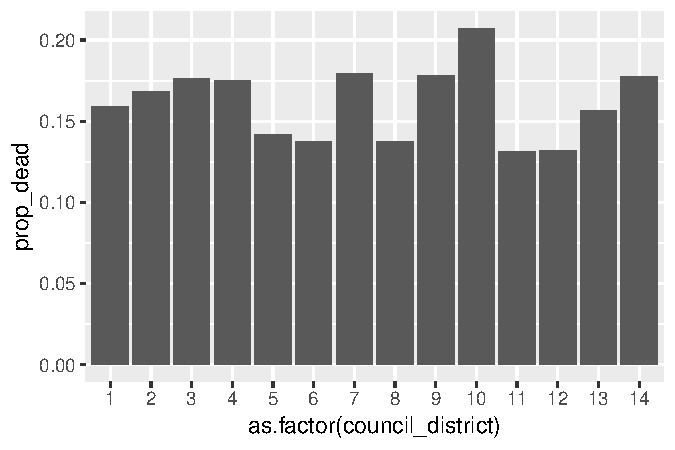
\includegraphics{Stage_3_files/figure-latex/unnamed-chunk-13-1.pdf}

Above you can see that certain city council districts have higher rates
of dogs dying in the shelter system. City council district 12 seems to
be the highest at 20.7\% of the dogs are dying in the shelter system,
and city council district 11 has the lowest at only 13.1\% of the dogs
dying in the shelter system.

\begin{Shaded}
\begin{Highlighting}[]
\NormalTok{just_dog_adoptions }\OperatorTok
\StringTok{  }\KeywordTok{group_by}\NormalTok{(council_district)}\OperatorTok
\StringTok{  }\KeywordTok{summarise}\NormalTok{(}\DataTypeTok{prop_adopted =} \KeywordTok{sum}\NormalTok{(adopted)}\OperatorTok{/}\KeywordTok{n}\NormalTok{())}\OperatorTok
\StringTok{  }\KeywordTok{filter}\NormalTok{(}\OperatorTok{!}\KeywordTok{is.na}\NormalTok{(council_district)) }\OperatorTok
\StringTok{  }\KeywordTok{ggplot}\NormalTok{(}\KeywordTok{aes}\NormalTok{(}\DataTypeTok{x=}\KeywordTok{as.factor}\NormalTok{(council_district), }\DataTypeTok{y =}\NormalTok{ prop_adopted)) }\OperatorTok{+}
\StringTok{  }\KeywordTok{geom_bar}\NormalTok{(}\DataTypeTok{stat =} \StringTok{"identity"}\NormalTok{)}
\end{Highlighting}
\end{Shaded}

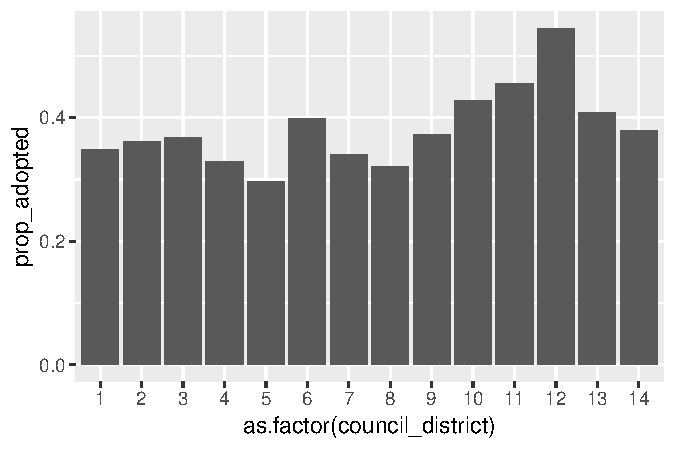
\includegraphics{Stage_3_files/figure-latex/unnamed-chunk-14-1.pdf}

For proportion adopted we see a range of values. City council district
12 has 54.5\% of the dogs adopted, while city council district 5 has the
lowest proportion adopted at only 0.297.

\subsubsection{Random Intercepts:}\label{random-intercepts}

\begin{Shaded}
\begin{Highlighting}[]
\NormalTok{mod.}\DecValTok{1}\NormalTok{=}\KeywordTok{glmer}\NormalTok{(adopted}\OperatorTok{~}\DecValTok{1}\OperatorTok{+}\NormalTok{(}\DecValTok{1}\OperatorTok{|}\NormalTok{council_district), }\DataTypeTok{data=}\NormalTok{just_dog_adoptions, }\DataTypeTok{family =} \StringTok{"binomial"}\NormalTok{)}
\KeywordTok{summary}\NormalTok{(mod.}\DecValTok{1}\NormalTok{)}
\end{Highlighting}
\end{Shaded}

\begin{verbatim}
## Generalized linear mixed model fit by maximum likelihood (Laplace
##   Approximation) [glmerMod]
##  Family: binomial  ( logit )
## Formula: adopted ~ 1 + (1 | council_district)
##    Data: just_dog_adoptions
## 
##      AIC      BIC   logLik deviance df.resid 
##  58685.9  58703.3 -29340.9  58681.9    45485 
## 
## Scaled residuals: 
##     Min      1Q  Median      3Q     Max 
## -1.0569 -0.7335 -0.6885  1.2963  1.5351 
## 
## Random effects:
##  Groups           Name        Variance Std.Dev.
##  council_district (Intercept) 0.05945  0.2438  
## Number of obs: 45487, groups:  council_district, 14
## 
## Fixed effects:
##             Estimate Std. Error z value Pr(>|z|)    
## (Intercept) -0.49300    0.06663  -7.399 1.37e-13 ***
## ---
## Signif. codes:  0 '***' 0.001 '**' 0.01 '*' 0.05 '.' 0.1 ' ' 1
\end{verbatim}

\begin{Shaded}
\begin{Highlighting}[]
\KeywordTok{exp}\NormalTok{(}\KeywordTok{fixef}\NormalTok{(mod.}\DecValTok{1}\NormalTok{))}\OperatorTok{/}\NormalTok{(}\DecValTok{1}\OperatorTok{+}\KeywordTok{exp}\NormalTok{(}\KeywordTok{fixef}\NormalTok{(mod.}\DecValTok{1}\NormalTok{)))}
\end{Highlighting}
\end{Shaded}

\begin{verbatim}
## (Intercept) 
##   0.3791861
\end{verbatim}

\begin{Shaded}
\begin{Highlighting}[]
\NormalTok{mod.1_dead=}\KeywordTok{glmer}\NormalTok{(out_dead}\OperatorTok{~}\DecValTok{1}\OperatorTok{+}\NormalTok{(}\DecValTok{1}\OperatorTok{|}\NormalTok{council_district), }\DataTypeTok{data=}\NormalTok{just_dog_adoptions, }\DataTypeTok{family =} \StringTok{"binomial"}\NormalTok{)}
\KeywordTok{summary}\NormalTok{(mod.1_dead)}
\end{Highlighting}
\end{Shaded}

\begin{verbatim}
## Generalized linear mixed model fit by maximum likelihood (Laplace
##   Approximation) [glmerMod]
##  Family: binomial  ( logit )
## Formula: out_dead ~ 1 + (1 | council_district)
##    Data: just_dog_adoptions
## 
##      AIC      BIC   logLik deviance df.resid 
##  39522.0  39539.5 -19759.0  39518.0    45485 
## 
## Scaled residuals: 
##     Min      1Q  Median      3Q     Max 
## -0.4909 -0.4592 -0.4080 -0.4014  2.4913 
## 
## Random effects:
##  Groups           Name        Variance Std.Dev.
##  council_district (Intercept) 0.01946  0.1395  
## Number of obs: 45487, groups:  council_district, 14
## 
## Fixed effects:
##             Estimate Std. Error z value Pr(>|z|)    
## (Intercept) -1.65465    0.04143  -39.94   <2e-16 ***
## ---
## Signif. codes:  0 '***' 0.001 '**' 0.01 '*' 0.05 '.' 0.1 ' ' 1
\end{verbatim}

\begin{Shaded}
\begin{Highlighting}[]
\KeywordTok{exp}\NormalTok{(}\KeywordTok{fixef}\NormalTok{(mod.1_dead))}\OperatorTok{/}\NormalTok{(}\DecValTok{1}\OperatorTok{+}\KeywordTok{exp}\NormalTok{(}\KeywordTok{fixef}\NormalTok{(mod.1_dead)))}
\end{Highlighting}
\end{Shaded}

\begin{verbatim}
## (Intercept) 
##   0.1604818
\end{verbatim}

\subsubsection{Multi-Level:}\label{multi-level}

\begin{Shaded}
\begin{Highlighting}[]
\NormalTok{mod.}\FloatTok{2.}\NormalTok{adopted=}\KeywordTok{glmer}\NormalTok{(adopted}\OperatorTok{~}\NormalTok{summer}\OperatorTok{+}\NormalTok{chip_status}\OperatorTok{+}\NormalTok{treatable_intake}\OperatorTok{+}\NormalTok{(}\DecValTok{1}\OperatorTok{|}\NormalTok{council_district), }\DataTypeTok{data=}\NormalTok{just_dog_adoptions, }\DataTypeTok{family =} \StringTok{"binomial"}\NormalTok{)}
\KeywordTok{summary}\NormalTok{(mod.}\FloatTok{2.}\NormalTok{adopted)}
\end{Highlighting}
\end{Shaded}

\begin{verbatim}
## Generalized linear mixed model fit by maximum likelihood (Laplace
##   Approximation) [glmerMod]
##  Family: binomial  ( logit )
## Formula: 
## adopted ~ summer + chip_status + treatable_intake + (1 | council_district)
##    Data: just_dog_adoptions
## 
##      AIC      BIC   logLik deviance df.resid 
##  57316.1  57359.7 -28653.0  57306.1    45482 
## 
## Scaled residuals: 
##     Min      1Q  Median      3Q     Max 
## -1.2426 -0.7608 -0.6787  1.2118  3.4802 
## 
## Random effects:
##  Groups           Name        Variance Std.Dev.
##  council_district (Intercept) 0.08389  0.2896  
## Number of obs: 45487, groups:  council_district, 14
## 
## Fixed effects:
##                  Estimate Std. Error z value Pr(>|z|)    
## (Intercept)      -1.93608    0.09252 -20.926  < 2e-16 ***
## summer            0.07182    0.02272   3.162  0.00157 ** 
## chip_status      -0.12224    0.02227  -5.490 4.03e-08 ***
## treatable_intake  1.59669    0.05142  31.050  < 2e-16 ***
## ---
## Signif. codes:  0 '***' 0.001 '**' 0.01 '*' 0.05 '.' 0.1 ' ' 1
## 
## Correlation of Fixed Effects:
##             (Intr) summer chp_st
## summer      -0.069              
## chip_status -0.073  0.027       
## treatbl_ntk -0.519  0.002 -0.014
\end{verbatim}

\begin{Shaded}
\begin{Highlighting}[]
\KeywordTok{exp}\NormalTok{(}\KeywordTok{fixef}\NormalTok{(mod.}\FloatTok{2.}\NormalTok{adopted))}
\end{Highlighting}
\end{Shaded}

\begin{verbatim}
##      (Intercept)           summer      chip_status treatable_intake 
##        0.1442687        1.0744612        0.8849374        4.9366449
\end{verbatim}

\begin{Shaded}
\begin{Highlighting}[]
\KeywordTok{exp}\NormalTok{(}\KeywordTok{fixef}\NormalTok{(mod.}\FloatTok{2.}\NormalTok{adopted))}\OperatorTok{/}\NormalTok{(}\DecValTok{1}\OperatorTok{+}\KeywordTok{exp}\NormalTok{(}\KeywordTok{fixef}\NormalTok{(mod.}\FloatTok{2.}\NormalTok{adopted)))}
\end{Highlighting}
\end{Shaded}

\begin{verbatim}
##      (Intercept)           summer      chip_status treatable_intake 
##        0.1260794        0.5179471        0.4694784        0.8315547
\end{verbatim}

\begin{Shaded}
\begin{Highlighting}[]
\NormalTok{mod.}\FloatTok{2.}\NormalTok{dead=}\KeywordTok{glmer}\NormalTok{(out_dead}\OperatorTok{~}\NormalTok{summer}\OperatorTok{+}\NormalTok{chip_status}\OperatorTok{+}\NormalTok{treatable_intake}\OperatorTok{+}\NormalTok{(}\DecValTok{1}\OperatorTok{|}\NormalTok{council_district), }\DataTypeTok{data=}\NormalTok{just_dog_adoptions, }\DataTypeTok{family =} \StringTok{"binomial"}\NormalTok{)}
\KeywordTok{summary}\NormalTok{(mod.}\FloatTok{2.}\NormalTok{dead)}
\end{Highlighting}
\end{Shaded}

\begin{verbatim}
## Generalized linear mixed model fit by maximum likelihood (Laplace
##   Approximation) [glmerMod]
##  Family: binomial  ( logit )
## Formula: 
## out_dead ~ summer + chip_status + treatable_intake + (1 | council_district)
##    Data: just_dog_adoptions
## 
##      AIC      BIC   logLik deviance df.resid 
##  36001.9  36045.5 -17996.0  35991.9    45482 
## 
## Scaled residuals: 
##     Min      1Q  Median      3Q     Max 
## -1.3865 -0.3979 -0.3527 -0.3135  3.4388 
## 
## Random effects:
##  Groups           Name        Variance Std.Dev.
##  council_district (Intercept) 0.01982  0.1408  
## Number of obs: 45487, groups:  council_district, 14
## 
## Fixed effects:
##                  Estimate Std. Error z value Pr(>|z|)    
## (Intercept)       0.08265    0.05258   1.572    0.116    
## summer            0.37470    0.02963  12.644  < 2e-16 ***
## chip_status      -0.23570    0.03116  -7.565 3.88e-14 ***
## treatable_intake -2.12055    0.03592 -59.039  < 2e-16 ***
## ---
## Signif. codes:  0 '***' 0.001 '**' 0.01 '*' 0.05 '.' 0.1 ' ' 1
## 
## Correlation of Fixed Effects:
##             (Intr) summer chp_st
## summer      -0.149              
## chip_status -0.194  0.020       
## treatbl_ntk -0.530 -0.051  0.021
\end{verbatim}

\begin{Shaded}
\begin{Highlighting}[]
\KeywordTok{exp}\NormalTok{(}\KeywordTok{fixef}\NormalTok{(mod.}\FloatTok{2.}\NormalTok{dead))}
\end{Highlighting}
\end{Shaded}

\begin{verbatim}
##      (Intercept)           summer      chip_status treatable_intake 
##        1.0861591        1.4545479        0.7900191        0.1199661
\end{verbatim}

\begin{Shaded}
\begin{Highlighting}[]
\KeywordTok{exp}\NormalTok{(}\KeywordTok{fixef}\NormalTok{(mod.}\FloatTok{2.}\NormalTok{dead))}\OperatorTok{/}\NormalTok{(}\DecValTok{1}\OperatorTok{+}\KeywordTok{exp}\NormalTok{(}\KeywordTok{fixef}\NormalTok{(mod.}\FloatTok{2.}\NormalTok{dead)))}
\end{Highlighting}
\end{Shaded}

\begin{verbatim}
##      (Intercept)           summer      chip_status treatable_intake 
##        0.5206502        0.5925930        0.4413468        0.1071159
\end{verbatim}


\end{document}
